\section{EXPERIMENTAL SETTING, RESULTS AND DISCUSSION}
\label{sec:exp}
\subsection{Experimental Setting}
The proposed framework for aging tolerance is implemented in C++ and the SAT-based formulation is solved by MiniSat on a 2.83GHz Intel Quad-Core CPU workstation running Linux. The benchmark circuits are chosen from the IWLS'05 and ISCAS'89 suites. The technology used is TSMC 45nm GP standard cell series.

Under 10-year BTI, the aging rates of clock buffers were obtained from HSPICE. The aging rates of clock buffers with duty cycles of 20\%, 40\%, 50\%, and 80\% are 8.51\%, 12.08\%, 13.51\%, and 16.41\% respectively and the aging rate of logic is obtained by using the predictive model presented in~\cite{wang2010impact},~\cite{wang2007efficient} (detailed in Section~\ref{subsec:apm}).


\begin{table*}
\centering
\caption{Benchmark information}
	%\begin{tabular}{l}
	%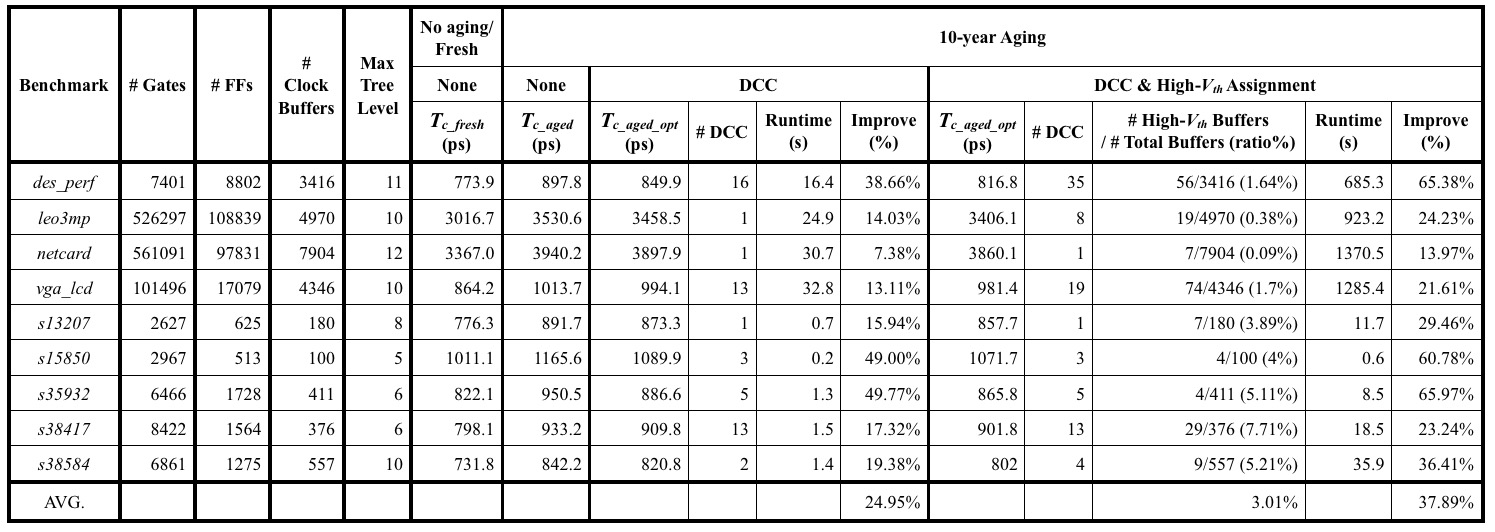
\includegraphics[width=2.03\columnwidth]{Experimental_result_DCC_TVA.png} %IEEE
	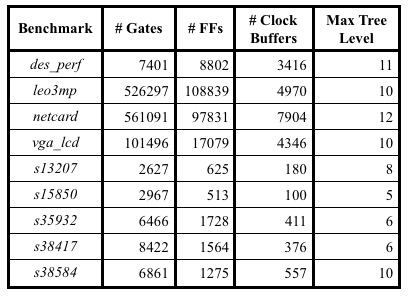
\includegraphics[width=0.47\columnwidth]{benchmark.png} %ACM
	%\end{tabular}
\label{table:exp1}
\end{table*}
\begin{table*}
\centering
\caption{Results of aging tolerance}
	%\begin{tabular}{l}
	%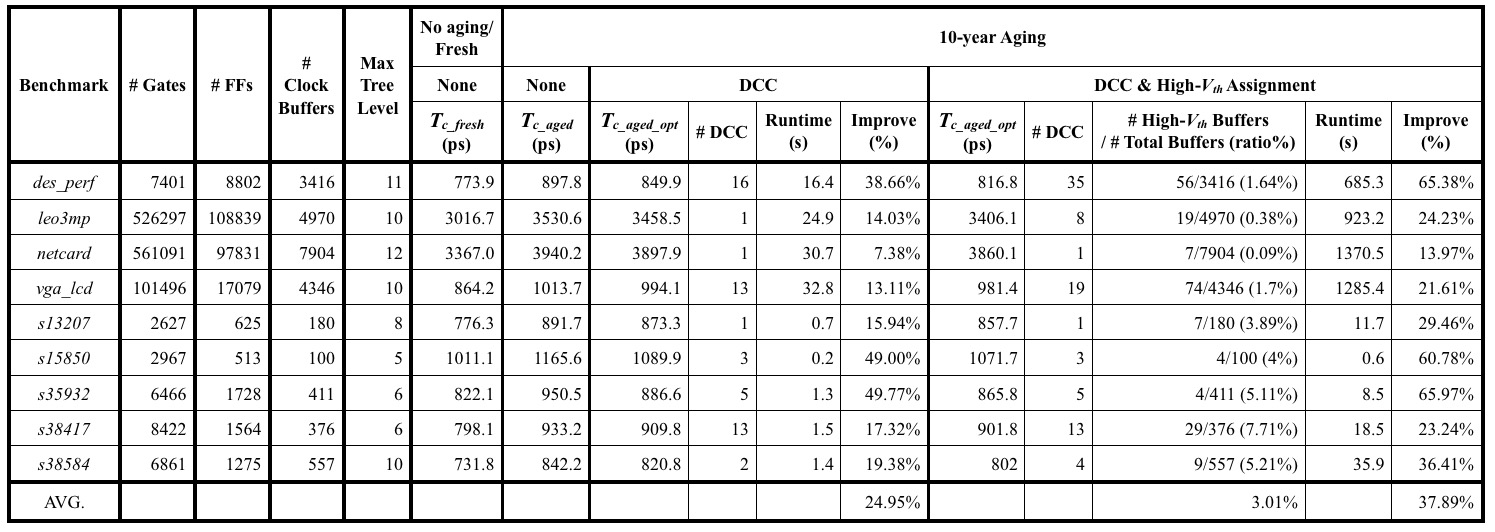
\includegraphics[width=2.03\columnwidth]{Experimental_result_DCC_TVA.png} %IEEE
	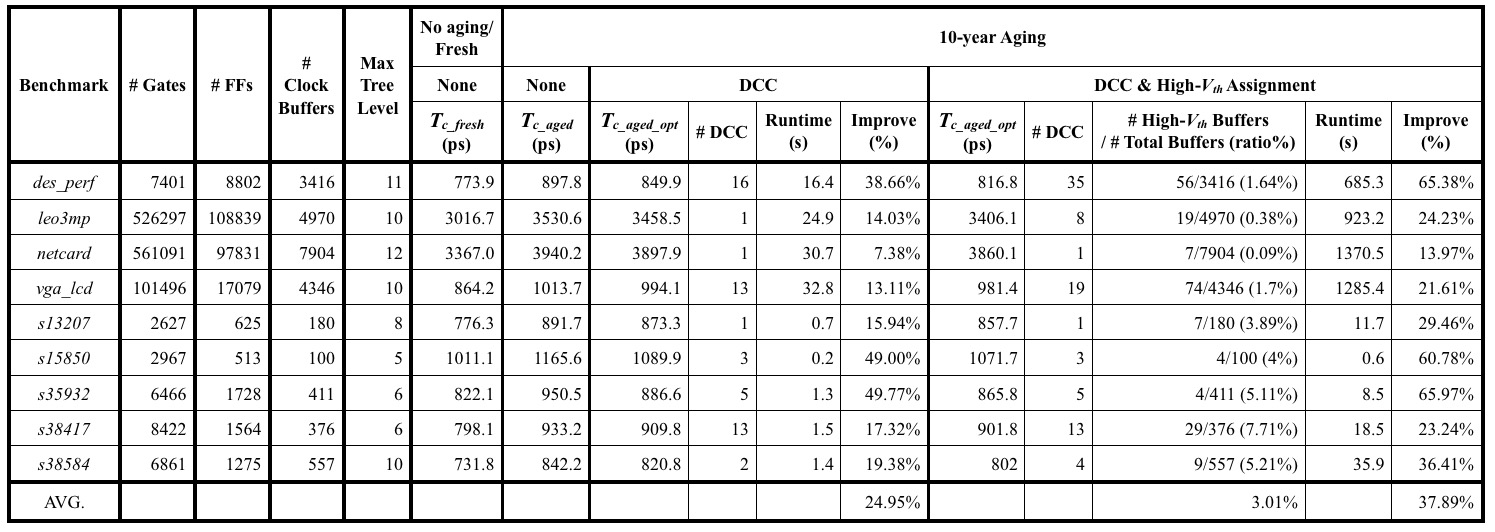
\includegraphics[width=1\columnwidth]{Experimental_result_DCC_TVA.png} %ACM
	%\end{tabular}
\label{table:exp2}
\end{table*}
\subsection{Experimental Results}
Table~\ref{table:exp1} and Table~\ref{table:exp2} reports the experimental results and information of each benchmark. In Table~\ref{table:exp1}, columns 2 to 5 show the total number of gates, total numbers of flip-flops, total numbers of clock buffers, and maximum level of the clock tree in each benchmark respectively. In Table~\ref{table:exp2}, column 2 demonstrates the fresh clock period that is the circuit delay without aging, denoted by $T_{c\_fresh}$. Column 3 demonstrates the clock period of the circuit under 10-year aging, denoted by $T_{c\_aged}$. Column 4 demonstrates the optimum clock period of the circuit under 10-year aging after applying our framework, denoted by $T_{c\_aged\_opt}$. A shorter clock period under aging implies better circuit performance and higher level of aging tolerance. Column 5 demonstrates the used DCC count. Column 6 demonstrates the runtime and the Column 7 demonstrates the improvement, i.e., the level of aging tolerance which is calculated as:
\begin{gather*}
1 - (T_{c\_aged\_opt} - T_{c\_fresh}) / (T_{c\_aged} - T_{c\_fresh})
\end{gather*}

For benchmark \textit{des\_perf}, $T_{c\_fresh}$ is 773.9ps and $T_{c\_aged}$ is 897.8ps, which means after 10-year aging the clock period of circuit will increase by 123.9ps. With DCC insertion using the proposed framework, the clock period achieved is 849.9ps, an increment of 76ps against $T_{c\_fresh}$ (38.66\% improvement). As shown in Table~\ref{table:exp2}, the improvement ranges from 7.38\% to 49.77\% and is 24.95\% on average. \iffalse As shown in Table~\ref{table:exp1}.\fi The number of inserted DCCs is between 2 (for benchmark \textit{s38584}) to 17 (for benchmark \textit{des\_perf}), implying very limited degree of circuit modification and insignificant design overhead. Moreover, as it can be seen in Column 12 to 16, when $V_{th}^h$ assignment for clock buffers is involved in the proposed framework, the resulting framework can give rise to lower clock periods, implying better improvement in aging tolerance. 

\subsection{Discussion: DCC Redeployment due to $V_{th}^h$ Assignment}
As we can see, the DCC counts in Column 13 are different from those in Column 9, implying that DCCs are redeployed in the clock tree while $V_{th}^h$ assignment is involved in the framework. More specifically, when $V_{th}^h$ assignment is considered, some clock buffers become candidate buffers to be inserted DCCs at their inputs, because timing constraints (i.e., setup-time and hold-time) are met based on the inequality Equation (1) and (2). In this way, DCCs can be redeployed to obtain lower clock periods, exploring better improvement in aging tolerance.


%Compare the DCC counts in Column 9 with those in Column 13, we can find that, while $V_{th}^h$ assignment is involved in the framework, it may redeploy the DCCs in the clock tree and thus results in different DCC count. Specifically speaking, when $V_{th}^h$ assignment is considered, some clock buffers become candidate buffers to be inserted DCCs at their inputs, because timing constraints (i.e., setup-time and hold-time) are met based on the inequality Equation (1) and (2). In this way, DCCs can be redeployed to obtain lower clock periods.

%Take \textit{des\_perf} for example, DCC count is 7; however, the DCC count increases to 33 after $V_{th}^h$ assignment is involved. The DCC counts of the same design differ because the DCC deployments are not identical anymore. Specifically speaking, when V\textsubscript{th} assignment is considered, some clock buffers become candidate buffers to be inserted DCC at their inputs, because timing constraints (i.e., setup-time and hold-time) are met based on the inequality Equation (1) and (2), such that DCC can be redeployed to obtain lower Tc. Thus, even thought the two frameworks target the identical benchmark, the DCC deployments/counts may differ. 

\subsection{Discussion: Increase in Runtime}
In addition, the run time of the framework, involving $V_{th}^h$ assignment, increases due to the possibility explosion of DCC deployment and leader selection. To be specific, given a pair of flip-flops and associated clock paths, we need to consider the various possibilities of leader selections, for each DCC deployment. Therefore, the total  count of DCC deployment and leader selection is equal to the combination of DCC deployment plus leader selection, i.e., DCC possibilities multiplied by the leader counterparts, accounting for the increase of run time. 

Even though the runtime increase while $V_{th}$ assignment is involved, the resulting framework is still practical for aging tolerance because it at most takes 1370 seconds for a comparative design (e.g., netcard).
\subsection{Discussion: Aging Impact on DCC}
\begin{figure}
    \centering
    %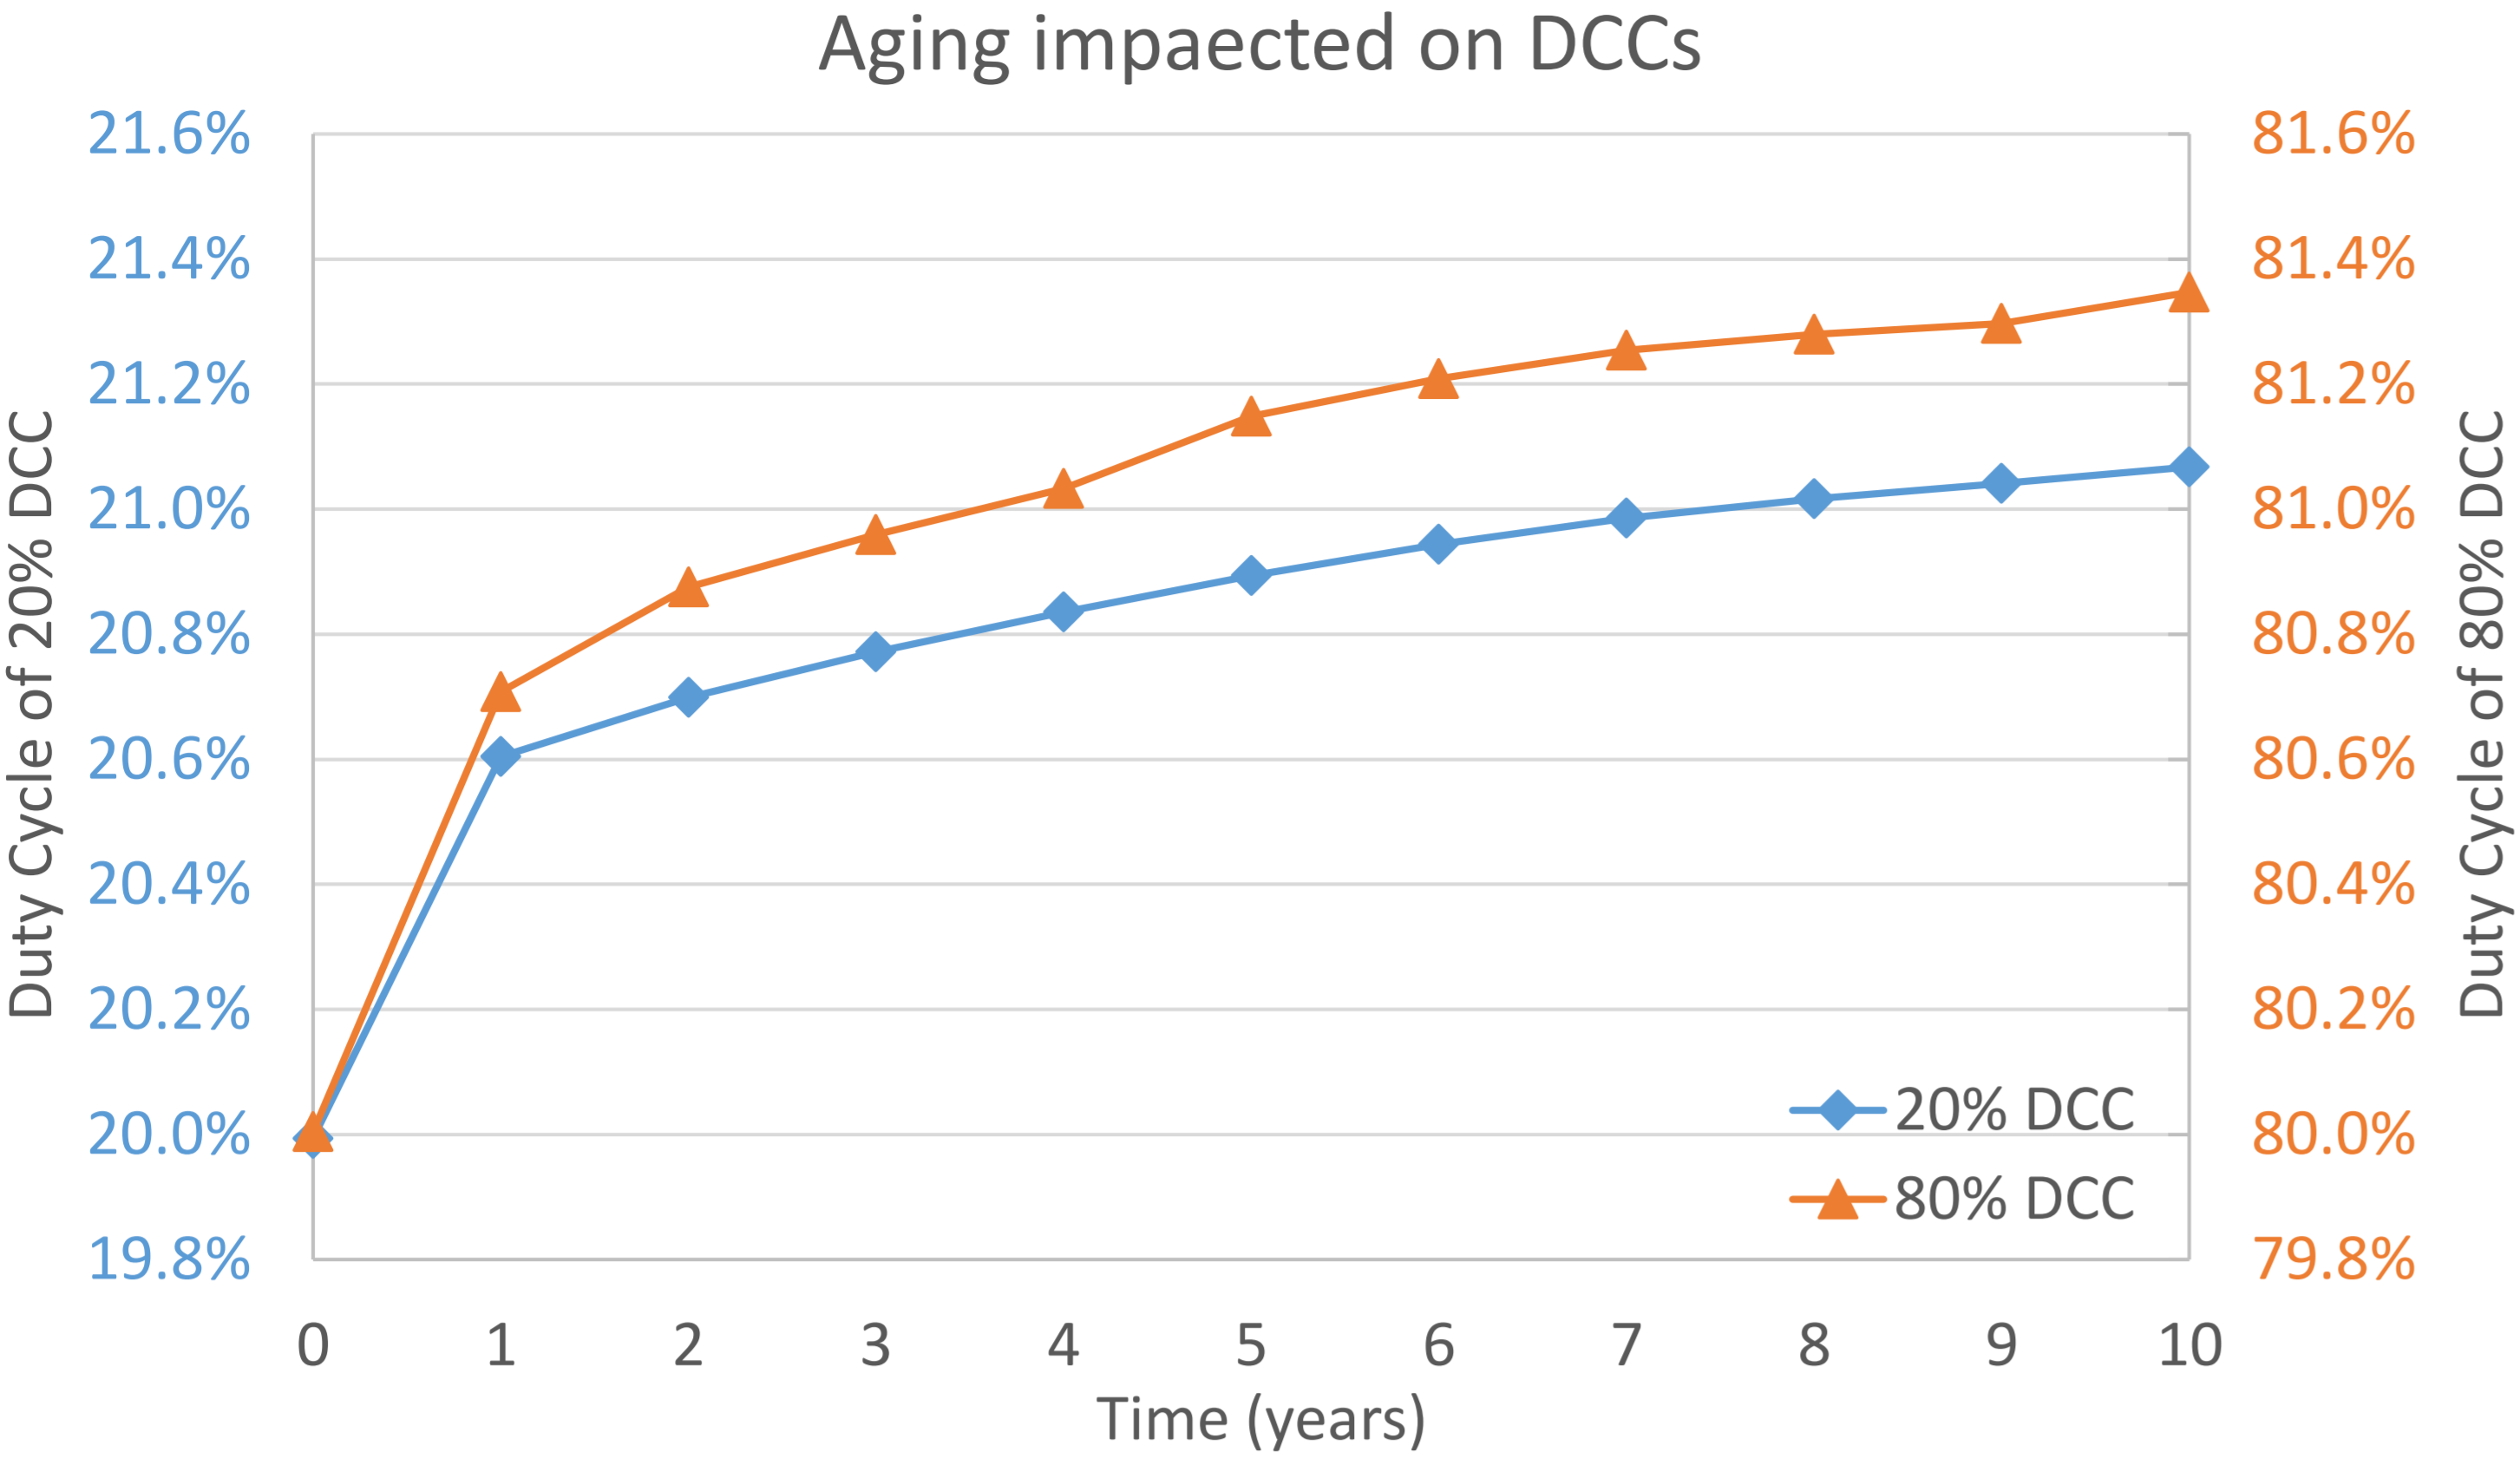
\includegraphics[width=0.9\columnwidth]{Aging_impacted_on_DCC.png} %IEEE
     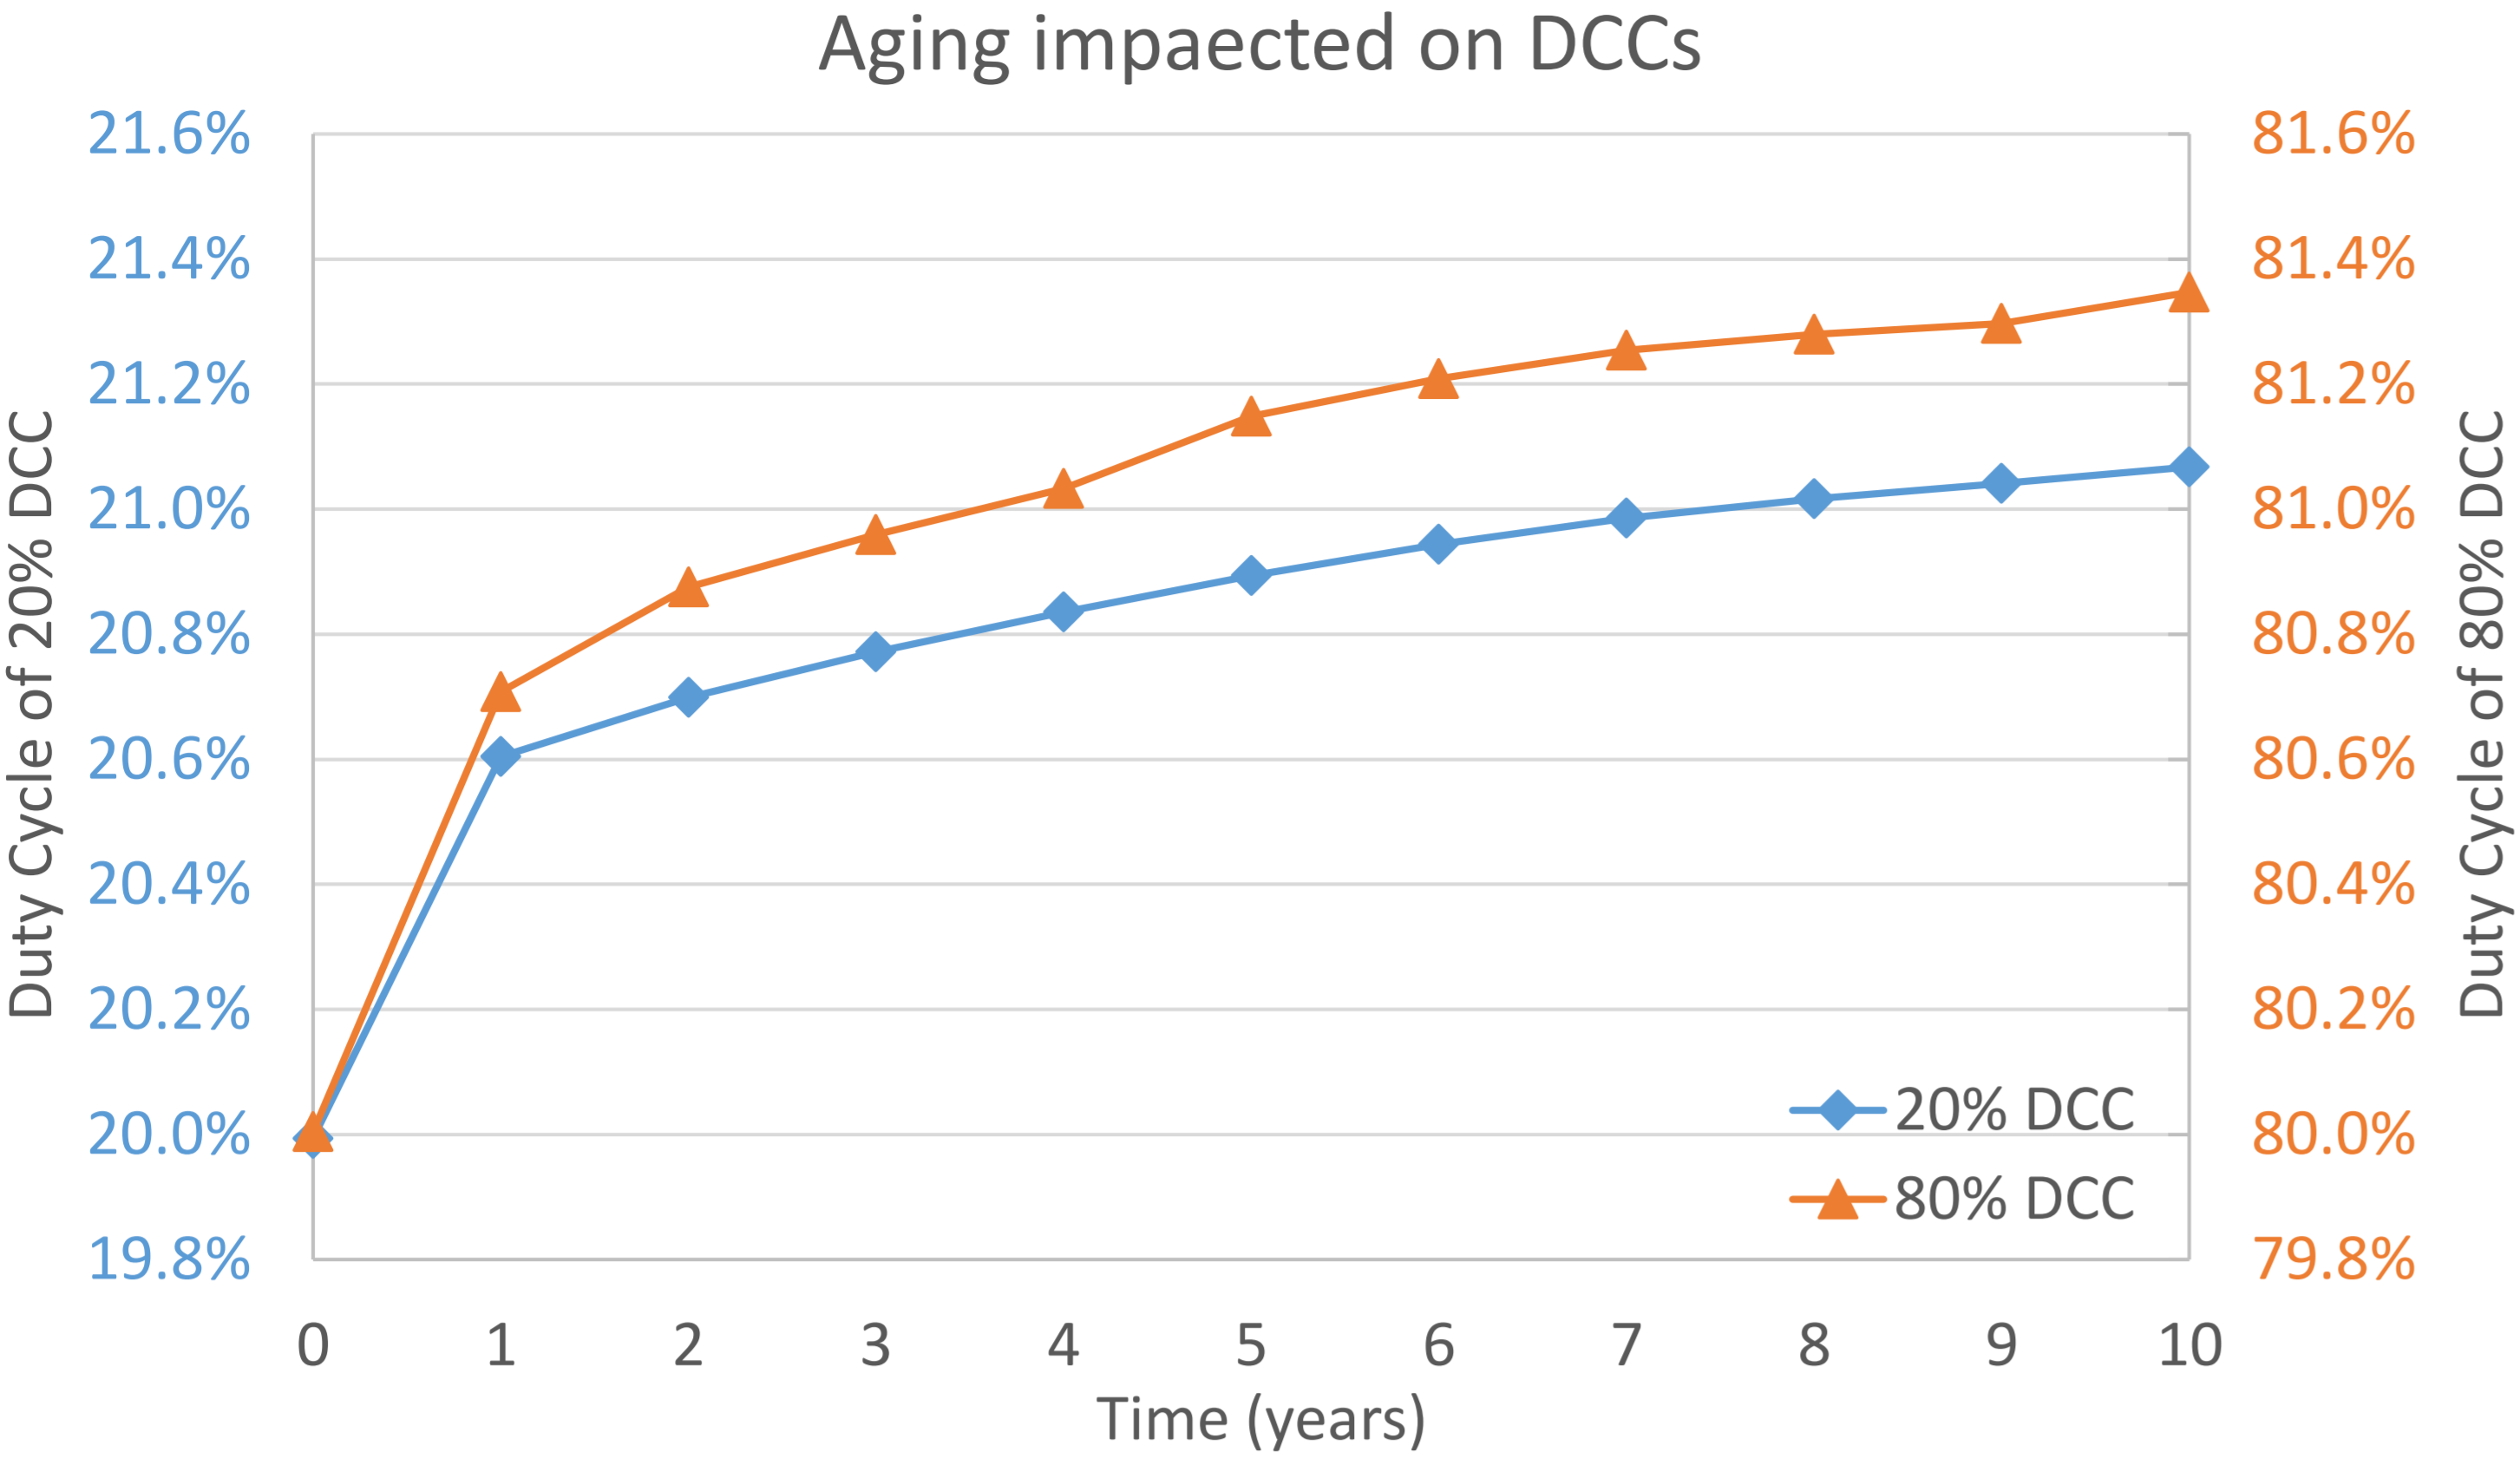
\includegraphics[width=0.6\columnwidth]{Aging_impacted_on_DCC.png} %ACM
    \caption{Aging impact on 20\%/80\% DCC under BTI}
    \label{fig:exp4}
\end{figure}

Figure~\ref{fig:exp4} shows the change in the duty cycle of a 20\%/80\% DCC over 10-year aging. The y axis on the left represents the duty cycle of a 20\% DCC, and the one on the right represents the duty cycle of an 80\% DCC. As it can be seen, the growth in both cases are marginal: $20\% \to 21.07\%$ for a 20\% DCC and $80\% \to 81.35\%$ for an 80\% DCC, which in turn should not affect the benefit of our proposed framework significantly.


\subsection{Discussion: Depth Boundary for DCC Deployment}
\begin{figure}
    \centering
    %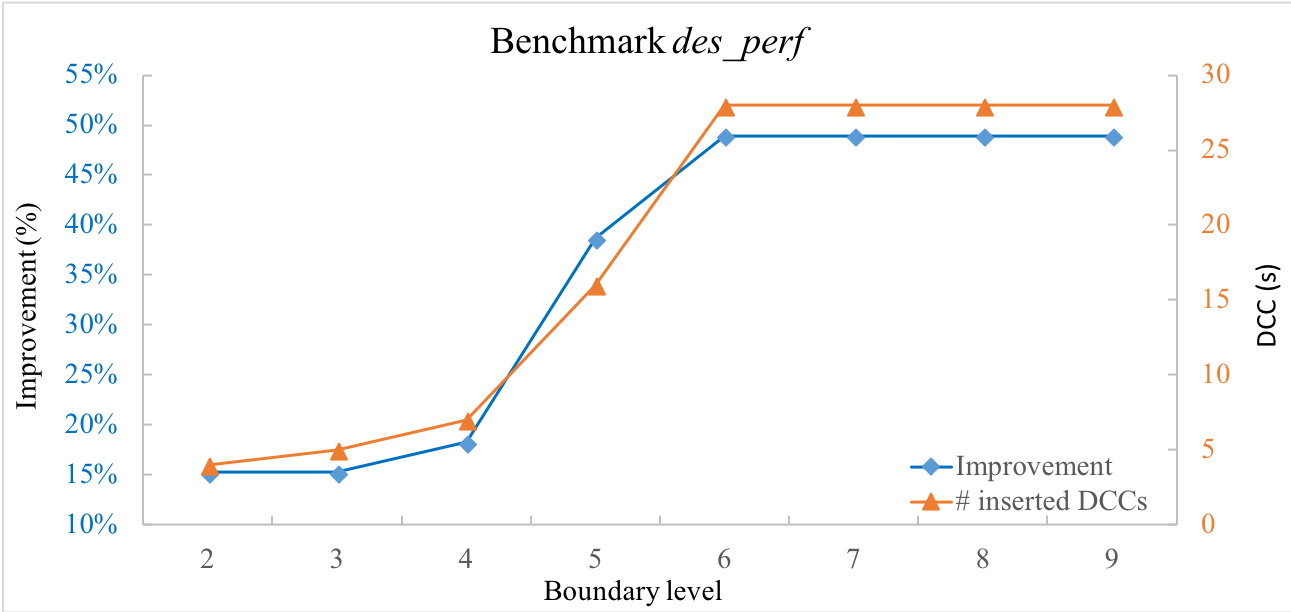
\includegraphics[width=0.9\columnwidth]{Boundary_level_vs_improvement.png} %IEEE
    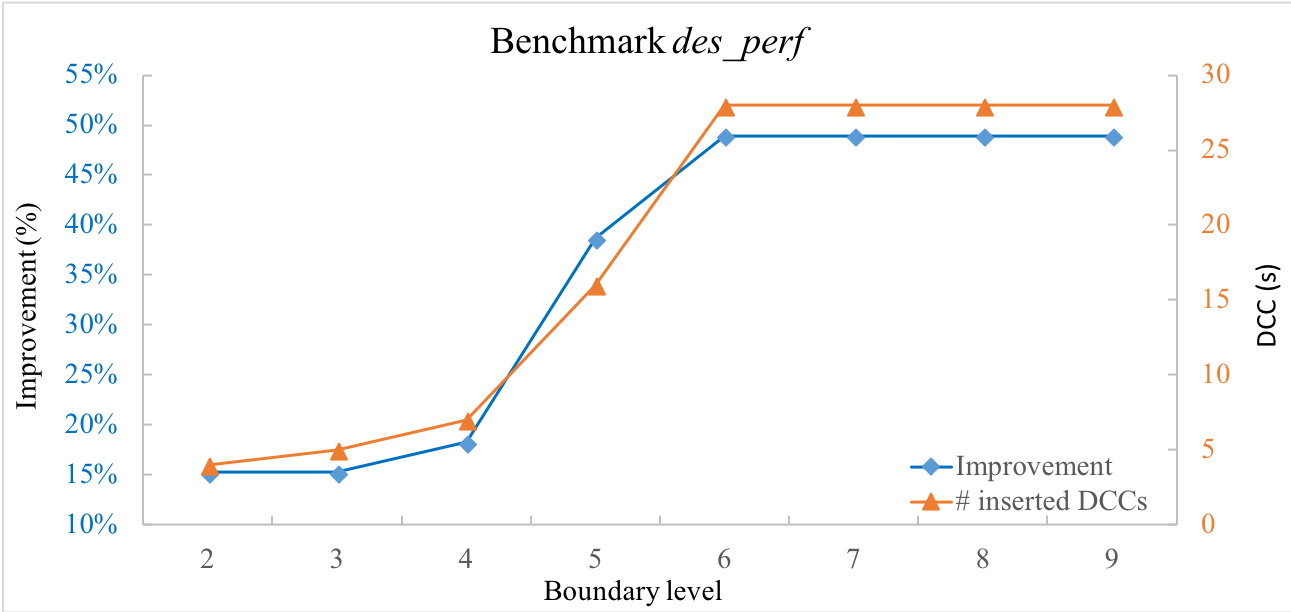
\includegraphics[width=0.6\columnwidth]{Boundary_level_vs_improvement.png} %ACM
    \caption{Improvement/Cost versus clock tree level considered}
    \label{fig:boundary}
\end{figure}

As mentioned in Section~\ref{sec:framework}, inserting DCCs deep in the clock tree is less effective. For benchmark \textit{des\_perf}, we considered the deployment of DCCs at the upper half of the clock tree (i.e., level 1 to 5) and achieved 38.66\% improvement in terms of aging tolerance. As demonstrated in Figure~\ref{fig:boundary}, if we expand the boundary of DCC deployment from level 1 in the clock tree to level 10 progressively, we can gain a considerable improvement from level 1 to 6; however, from 7 to 10, the improvement become stagnant, but more DCCs are required.